%%%%%%%%%%%%%%%%%%%%%%%%%%%%%%%%%%%%%%%%%%%%%%%%%%%%%%%%%%%%%%%%%%%%%%%%%%%%%%%%%%
\begin{frame}[fragile]\frametitle{}
\begin{center}
{\Large Introduction}
\end{center}
\end{frame}

%%%%%%%%%%%%%%%%%%%%%%%%%%%%%%%%%%%%%%%%%%%%%%%%%%%%%%%%%%%%%%%%%%%%%%%%%%%%%%%%%%
\begin{frame}[fragile]\frametitle{Future AI?}
  \begin{itemize}
    \item What are future AI applications like?
	\begin{itemize}
		\item Generative: Generate content like text \& image
		\item Agentic: Execute complex tasks on behalf of human
	 \end{itemize}
	\item How do we empower every developer to build them?: 
	\begin{itemize}
		\item Co-Pilots
		\item Autonomous
	 \end{itemize}	
  \end{itemize}
\end{frame}

%%%%%%%%%%%%%%%%%%%%%%%%%%%%%%%%%%%%%%%%%%%%%%%%%%%%%%%%%%%%%%%%%%%%%%%%%%%%%%%%%%
\begin{frame}[fragile]\frametitle{Introduction to AI Agents}
    \begin{itemize}
        \item 2024 is expected to be the year of AI agents.
        \item AI agents combine multiple components to solve complex problems.
        \item Shifting from monolithic models to compound AI systems.
        \item Compound AI systems use system design for better problem solving.
        \item AI agents improve with reasoning, acting, and memory components. (ReAct = Reasoning + Acting)
    \end{itemize}
\end{frame}

%%%%%%%%%%%%%%%%%%%%%%%%%%%%%%%%%%%%%%%%%%%%%%%%%%%%%%%%%%%%%%%%%%%%%%%%%%%%%%%%%%
\begin{frame}[fragile]\frametitle{From Monolithic Models to Compound AI}
    \begin{itemize}
        \item Monolithic models are limited by training data.
        \item Hard to adapt without significant data and resources.
        \item Example: Vacation planning with no personal data access.
        \item Compound AI systems solve this by integrating multiple components.
        \item External databases and tools enhance model responses.
    \end{itemize}
\end{frame}

%%%%%%%%%%%%%%%%%%%%%%%%%%%%%%%%%%%%%%%%%%%%%%%%%%%%%%%%%%%%%%%%%%%%%%%%%%%%%%%%%%
\begin{frame}[fragile]\frametitle{System Design in Compound AI}
    \begin{itemize}
        \item Systems are modular: combine models, tools, and databases.
        \item Easier to adapt and quicker to solve problems.
        \item Combining models with external components for enhanced output.
        \item Example: Search query integrated with model for better accuracy.
        \item Programmatic control logic guides the response.
    \end{itemize}
\end{frame}

%%%%%%%%%%%%%%%%%%%%%%%%%%%%%%%%%%%%%%%%%%%%%%%%%%%%%%%%%%%%%%%%%%%%%%%%%%%%%%%%%%
\begin{frame}[fragile]\frametitle{Role of Agents in Compound AI}
    \begin{itemize}
        \item Agents use large language models (LLMs) for reasoning and planning.
        \item LLMs break down problems into manageable tasks.
        \item Slow thinking (planning) leads to better solutions.
        \item Agents provide flexibility in solving complex tasks.
        \item The agent's role is to manage logic and interact with tools.
    \end{itemize}
\end{frame}

%%%%%%%%%%%%%%%%%%%%%%%%%%%%%%%%%%%%%%%%%%%%%%%%%%%%%%%%%%%%%%%%%%%%%%%%%%%%%%%%%%
\begin{frame}[fragile]\frametitle{Components of LLM Agents}
    \begin{itemize}
        \item Reasoning: Break down complex problems into steps.
        \item Acting: Use external tools like databases or calculators.
        \item Memory: Store logs and conversation history for personalization.
        \item Tools: External programs that help solve problems (e.g., search, calculators).
        \item Configurations: Adjust agents using frameworks like ReACT.
    \end{itemize}
\end{frame}

%%%%%%%%%%%%%%%%%%%%%%%%%%%%%%%%%%%%%%%%%%%%%%%%%%%%%%%%%%%%%%%%%%%%%%%%%%%%%%%%%%
\begin{frame}[fragile]\frametitle{Example: REACT Agent in Action}
    \begin{itemize}
        \item REACT agents think slowly, plan, and act iteratively.
        \item User query feeds into the agent with reasoning instructions.
        \item The agent may call external tools and evaluate the results.
        \item If the result is wrong, the agent revises its plan.
        \item Example: Calculating sunscreen needs for a vacation.
    \end{itemize}
\end{frame}

%%%%%%%%%%%%%%%%%%%%%%%%%%%%%%%%%%%%%%%%%%%%%%%%%%%%%%%%%%%%%%%%%%%%%%%%%%%%%%%%%%
\begin{frame}[fragile]\frametitle{Modularity and Complex Problem Solving}
    \begin{itemize}
        \item Modular AI systems can solve more complex problems.
        \item Example: Planning vacation with weather, sunscreen, and health data.
        \item Agents handle multiple paths to find the best solution.
        \item Compound AI is flexible and adapts to different problem scopes.
    \end{itemize}
\end{frame}

%%%%%%%%%%%%%%%%%%%%%%%%%%%%%%%%%%%%%%%%%%%%%%%%%%%%%%%%%%%%%%%%%%%%%%%%%%%%%%%%%%
\begin{frame}[fragile]\frametitle{Agent Autonomy in Problem Solving}
    \begin{itemize}
        \item Narrow problems can be solved with fixed, programmatic systems.
        \item Complex tasks require agent autonomy for better flexibility.
        \item Autonomy level depends on task complexity and need for iteration.
        \item Agents are effective for complex, diverse tasks (e.g., GitHub issues).
    \end{itemize}
\end{frame}

%%%%%%%%%%%%%%%%%%%%%%%%%%%%%%%%%%%%%%%%%%%%%%%%%%%%%%%%%%%%%%%%%%%%%%%%%%%%%%%%%%
\begin{frame}[fragile]\frametitle{The Future of Agent Systems}
    \begin{itemize}
        \item AI agents are evolving rapidly with system design and autonomy.
        \item Human-in-the-loop still essential for accuracy in early stages.
        \item Agents will play a key role in diverse industries and tasks.
        \item Expect increasing adoption in 2024 and beyond.
    \end{itemize}
\end{frame}


%%%%%%%%%%%%%%%%%%%%%%%%%%%%%%%%%%%%%%%%%%%%%%%%%%%%%%%%%%%%%%%%%%%%%%%%%%%%%%%%%%
\begin{frame}[fragile]\frametitle{Examples of Agentic AI}
  \begin{itemize}
  \item Agents mean ACTION
  \item Agentic AI means ACTION using AI, meaning LLM
  \item Examples:
  \begin{itemize}
    \item Personal assistants
    \item Autonomous robots
    \item Gaming agents
    \item Science agents
    \item Web agents
    \item Software agents
  \end{itemize}
    \end{itemize}

\end{frame}


%%%%%%%%%%%%%%%%%%%%%%%%%%%%%%%%%%%%%%%%%%%%%%%%%%%%%%%%%%%%%%%%%%%%%%%%%%%%%%%%%%
\begin{frame}[fragile]\frametitle{Autonomous AI Agents}
  \begin{itemize}
    \item Collaborative approach yields astonishing enhancements in performance and capabilities. Contrasted with using a single AI, such as ChatGPT, in isolation.
    \item Ability to assume distinct roles within a team. Like professionals in various fields.
    \item Each agent contributes specialized expertise to the conversation.
  \end{itemize}
\end{frame}

%%%%%%%%%%%%%%%%%%%%%%%%%%%%%%%%%%%%%%%%%%%%%%%%%%%%%%%%%%%%%%%%%%%%%%%%%%%%%%%%%%
\begin{frame}[fragile]\frametitle{The Blueprint}
  \begin{itemize}
    \item Planning: Reflects on past experiences, offers self-critiques, and breaks down tasks into manageable steps using sub-goal decomposition.
    \item Memory: Utilizes sensory, short-term, and long-term memory for real-time data processing, task-specific information, and retaining knowledge/experiences.
    \item Tools: Equipped with a virtual toolbox, accessing calendars, calculators, search engines, and other resources for versatile problem-solving.
  \end{itemize}
\end{frame}

%%%%%%%%%%%%%%%%%%%%%%%%%%%%%%%%%%%%%%%%%%%%%%%%%%%%%%%%%%%%%%%%%%%%%%%%%%%%%%%%%%
\begin{frame}[fragile]\frametitle{Flow: The Symphony}
  \begin{itemize}
    \item Task Decomposition % : Breaks down tasks into smaller, more manageable components for enhanced efficiency and accuracy.
    \item Model (LLM) Selection % : Chooses the most suitable Large Language Model (LLM) for the task to align actions with desired outcomes.
    \item Task Execution leveraging planning, memory, and tools.
    \item Response Generation % : Generates contextually relevant and accurate responses, be it drafting a report, answering questions, or making decisions.
  \end{itemize}
\end{frame}

%%%%%%%%%%%%%%%%%%%%%%%%%%%%%%%%%%%%%%%%%%%%%%%%%%%%%%%%%%%%%%%%%%%%%%%%%%%%%%%%%%
\begin{frame}[fragile]\frametitle{Agentic Frameworks' Needs}

  \begin{itemize}
  \item Intuitive unified agentic abstraction
  \item Flexible multi-agent orchestration
  \item Effective implementation of agentic design patterns
  \item Support diverse application needs
    \item  Handle more complex tasks / Improve response quality
	\item Easy to understand, maintain, extend Modular composition, Natural human participation, Fast \& creative experimentation
	  \item Agentic Abstraction: Unify models, tools, human for compound AI systems

  \end{itemize}
\end{frame}

%%%%%%%%%%%%%%%%%%%%%%%%%%%%%%%%%%%%%%%%%%%%%%%%%%%%%%%%%%%%%%%%%%%%%%%%%%%%%%%%%%
\begin{frame}[fragile]\frametitle{Multi-Agent Orchestration}


\begin{columns}
    \begin{column}[T]{0.6\linewidth}

		  \begin{itemize}
		  \item Static/dynamic
		  \item Context sharing/isolation
		  \item Cooperation/competition
		  \item Centralized/decentralized
		  \item Intervention/automation
		  \end{itemize}

    \end{column}
    \begin{column}[T]{0.4\linewidth}

		\begin{center}
		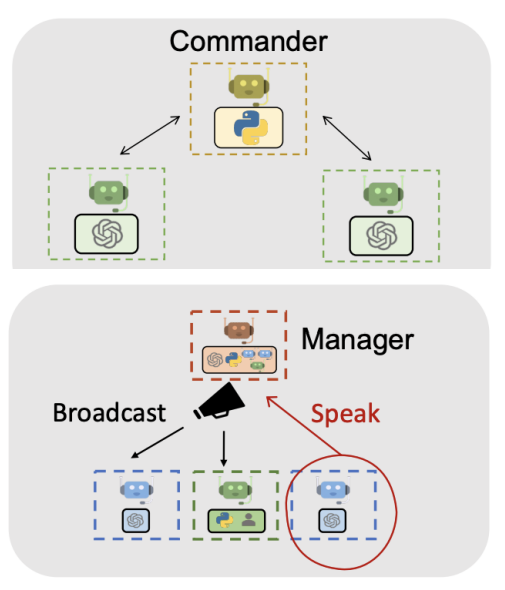
\includegraphics[width=\linewidth,keepaspectratio]{autoagent4}
		\end{center}
	
    \end{column}
  \end{columns}
  
  

\end{frame}

%%%%%%%%%%%%%%%%%%%%%%%%%%%%%%%%%%%%%%%%%%%%%%%%%%%%%%%%%%%%%%%%%%%%%%%%%%%%%%%%%%
\begin{frame}[fragile]\frametitle{Popular Agentic Frameworks}

  \begin{itemize}
    \item BabyAGI: Pioneering AI learning system.
    \item AutoGPT: Automates content generation.
    \item GPT Engineer: Assists in coding and software development.
	\item Langgraph: Graph-based control flow
	\item CrewAI: High-level static agent-task workflow
    \item AutoGen: Dialog based planning and execution
  \end{itemize}
\end{frame}

%%%%%%%%%%%%%%%%%%%%%%%%%%%%%%%%%%%%%%%%%%%%%%%%%%%%%%%%%%%%%%%%%%%%%%%%%%%%%%%%%%
\begin{frame}[fragile]\frametitle{LangGraph}
\begin{itemize}
    \item Open-source framework by \textbf{Langchain} for stateful, multi-actor applications.
    \item Inspired by \textbf{directed acyclic graphs (DAGs)} for data processing pipelines.
    \item Treats workflows as graphs with \textbf{nodes for specific tasks or functions}.
    \item Enables \textbf{fine-grained control} over application flow and state.
    \item Suitable for \textbf{complex workflows} with advanced memory and error recovery.
    \item Supports \textbf{human-in-the-loop} interactions.
    \item Integrates with \textbf{LangChain} for tools and models.
    \item Supports \textbf{multi-agent interaction patterns}.
\end{itemize}
\end{frame}

%%%%%%%%%%%%%%%%%%%%%%%%%%%%%%%%%%%%%%%%%%%%%%%%%%%%%%%%%%%%%%%%%%%%%%%%%%%%%%%%%%
\begin{frame}[fragile]\frametitle{Autogen}
\begin{itemize}
    \item Framework by \textbf{Microsoft} for building conversational agents.
    \item Treats workflows as \textbf{conversations between agents}.
    \item Intuitive for users preferring \textbf{ChatGPT-like interfaces}.
    \item Supports tools like \textbf{code executors} and \textbf{function callers}.
    \item Allows agents to perform \textbf{complex tasks autonomously}.
    \item Highly \textbf{customizable} for additional components and custom workflows.
    \item \textbf{Modular design}: Easy to maintain.
    \item Suitable for \textbf{simple and complex multi-agent scenarios}.
\end{itemize}
\end{frame}

%%%%%%%%%%%%%%%%%%%%%%%%%%%%%%%%%%%%%%%%%%%%%%%%%%%%%%%%%%%%%%%%%%%%%%%%%%%%%%%%%%
\begin{frame}[fragile]\frametitle{Crew AI}
\begin{itemize}
    \item Framework for \textbf{collaboration of role-based AI agents}.
    \item Agents are assigned \textbf{specific roles and goals}.
    \item Ideal for \textbf{sophisticated multi-agent systems}.
    \item Examples: \textbf{Multi-agent research teams}.
    \item Supports \textbf{flexible task management} and delegation.
    \item Enables \textbf{autonomous inter-agent collaboration}.
    \item Provides \textbf{customizable tools} for diverse applications.
\end{itemize}
\end{frame}

%%%%%%%%%%%%%%%%%%%%%%%%%%%%%%%%%%%%%%%%%%%%%%%%%%%%%%%%%%%%%%%%%%%%%%%%%%%%%%%%%%
\begin{frame}[fragile]\frametitle{Ease of Usage}
\begin{itemize}
    \item \textbf{Ease of usage} impacts learning curve and deployment time.
    \item \textbf{LangGraph:} Uses graphs (DAGs), ideal for pipeline users but needs graph understanding.
    \item \textbf{Autogen:} Uses conversations, intuitive for chat-based tasks, simplifies interaction management.
    \item \textbf{Crew AI:} Role-based design, agents act as cohesive units, easy to start.
\end{itemize}
\end{frame}

%%%%%%%%%%%%%%%%%%%%%%%%%%%%%%%%%%%%%%%%%%%%%%%%%%%%%%%%%%%%%%%%%%%%%%%%%%%%%%%%%%
\begin{frame}[fragile]\frametitle{Tool Coverage}
\begin{itemize}
    \item \textbf{Tool coverage} expands agent capabilities through supported functionalities.
    \item \textbf{LangGraph:} Integrates with LangChain for tool calling, memory, and human-in-the-loop interactions.
    \item \textbf{Autogen:} Supports tools like code executors and function callers; modular design eases new tool integration.
    \item \textbf{Crew AI:} Built over LangChain, inherits their tools; allows defining and integrating custom tools.
\end{itemize}
\end{frame}

%%%%%%%%%%%%%%%%%%%%%%%%%%%%%%%%%%%%%%%%%%%%%%%%%%%%%%%%%%%%%%%%%%%%%%%%%%%%%%%%%%
\begin{frame}[fragile]\frametitle{Memory Support}
\begin{itemize}
    \item \textbf{Memory Support:} Enables agents to maintain context for coherent interactions.
    \item \textbf{Types of Memory:}
    \begin{itemize}
        \item \textbf{Short-Term Memory:} Recalls recent interactions relevant to current tasks.
        \item \textbf{Long-Term Memory:} Preserves insights from past interactions for knowledge building.
        \item \textbf{Entity Memory:} Organizes data on specific entities for deeper understanding.
        \item \textbf{Contextual Memory:} Combines all memory types to sustain interaction context.
    \end{itemize}
    \item \textbf{LangGraph:} Offers advanced memory features, including short-term, long-term, and entity memory. Supports error recovery and time travel.
    \item \textbf{Autogen:} Uses a conversation-driven approach to maintain context across tasks.
    \item \textbf{Crew AI:} Provides comprehensive memory systems, ensuring contextual consistency and knowledge retention.
\end{itemize}
\end{frame}

%%%%%%%%%%%%%%%%%%%%%%%%%%%%%%%%%%%%%%%%%%%%%%%%%%%%%%%%%%%%%%%%%%%%%%%%%%%%%%%%%%
\begin{frame}[fragile]\frametitle{Structured Output}
\begin{itemize}
    \item \textbf{Structured Output:} Ensures responses are well-organized and interpretable.
    \item \textbf{Benefits:}
    \begin{itemize}
        \item Facilitates further processing and analysis.
        \item Enhances workflow management.
    \end{itemize}
    \item \textbf{LangGraph:} Nodes return structured output for workflow routing and state updates.
    \item \textbf{Autogen:} Supports structured responses via function-calling capabilities.
    \item \textbf{Crew AI:} Allows parsing outputs as Pydantic models or JSON, enabling custom-defined output structures.
\end{itemize}
\end{frame}

%%%%%%%%%%%%%%%%%%%%%%%%%%%%%%%%%%%%%%%%%%%%%%%%%%%%%%%%%%%%%%%%%%%%%%%%%%%%%%%%%%
\begin{frame}[fragile]\frametitle{Multi-Agent Support}
\begin{itemize}
    \item \textbf{Multi-Agent Support:} Handles diverse interaction patterns between agents.
    \item \textbf{Key Features:}
    \begin{itemize}
        \item Supports hierarchical, sequential, and dynamic patterns.
        \item Enables focused tasks by grouping tools and responsibilities.
        \item Allows separate prompts for better task execution.
        \item Agents can use distinct fine-tuned LLMs for improved functionality.
    \end{itemize}
    \item \textbf{LangGraph:} Supports hierarchical and dynamic interactions with graph-based visualization. 
    \begin{itemize}
        \item Provides flexibility through explicit agent definitions and transition probabilities.
        \item Best for constructing complex workflows.
    \end{itemize}
    \item \textbf{Autogen:} Treats workflows as agent conversations.
    \begin{itemize}
        \item Enables sequential and nested chats for dynamic interactions.
        \item Easy to manage complex collaborations.
    \end{itemize}
    \item \textbf{Crew AI:} Focuses on role-based interactions and autonomous delegation.
    \begin{itemize}
        \item Implements hierarchical and sequential task execution.
        \item Creates cohesive multi-agent teams.
    \end{itemize}
\end{itemize}
\end{frame}

%%%%%%%%%%%%%%%%%%%%%%%%%%%%%%%%%%%%%%%%%%%%%%%%%%%%%%%%%%%%%%%%%%%%%%%%%%%%%%%%%%
\begin{frame}[fragile]\frametitle{Summary}
		\begin{center}
		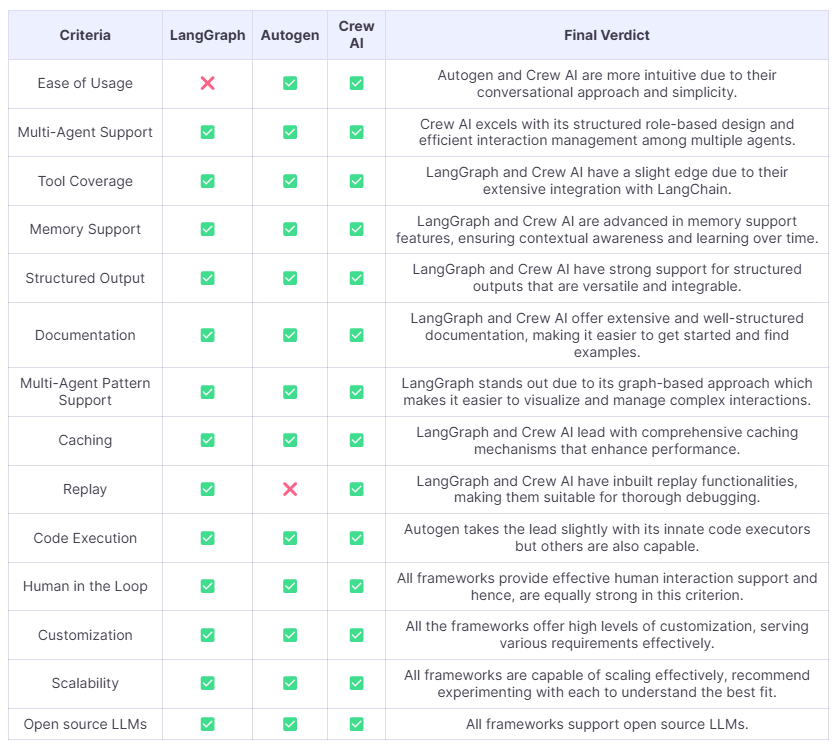
\includegraphics[width=0.8\linewidth,keepaspectratio]{autoagent14}
		\end{center}
		
		{\tiny (Ref: Mastering Agents: LangGraph Vs Autogen Vs Crew AI - Pratik Bhavsar)}
\end{frame}